\documentclass{beamer}
\usepackage[utf8]{inputenc}
\usepackage{graphicx}
\usetheme{default}
\usecolortheme{default}

\title[S03 Extensions MLS]{Section 03 : Extensions au modèle linéaire simple\\ (Séance 7)}
\subtitle{GSF-6053: Économétrie Financière}
\author[SP. Boucher]{Simon-Pierre Boucher\inst{1}}
\institute[Université Laval]
{
  \inst{1}%
  Département de finance, assurance et immobilier\\
  Faculté des sciences de l'administration\\
  Université Laval}
\date[Hiver 2022]{22 février 2022}

\begin{document}

\begin{frame}
  \titlepage
\end{frame}

\begin{frame}{Références}
\textbf{Obligatoires:}
\begin{itemize}
\item \textbf{Notes de cours:} Section 3 (Professeure: Marie-Hélène Gagnon)
\item \textbf{Woolridge:} chapitres 3, 8, 12.
\end{itemize}
\vspace{0.5cm}
\textbf{Complémentaires:}
\begin{itemize}
\item \textbf{Gujarati et Porter:} chapitres 10, 11, 12, 13 et appendice C.
\item \textbf{Greene:} chapitres 2, 3, 4, 5, 9, 14, 20 C et D
\end{itemize}
\end{frame}


\begin{frame}{Plan de la séance}
  \tableofcontents
\end{frame}

\section{Autocorrélation des erreurs}

\frame{\tableofcontents[current]}


\begin{frame}{Autocorrélation des erreurs}
\begin{itemize}
\item L’autocorrélation ou la corrélation sérielle des erreurs dans les séries chronologiques est assez fréquente. 
\item Elle découle souvent du fait qu’il y a une certaine « inertie » dans les données économiques et financières, c’est-à-dire que les observations passées se reflètent souvent dans les observations présentes et futures. 
\item Cela peut amener des problèmes de corrélation sérielle des erreurs si une variable autocorrelée est omise du modèle, par exemple.
\item Il est important de s’assurer lorsque vous détecter de l’autocorrélation qu’elle n’est pas dû à la non-stationnarité de Y et X. 
\item En effet, si ces deux quantités sont non stationnaires, les erreurs le seront possiblement aussi et seront possiblement autocorrelées.

\end{itemize}
\end{frame}

\begin{frame}{Autocorrélation des erreurs}
\begin{itemize}
\item Même si le modèle est bien spécifié, on peut penser que les erreurs (les chocs) affectant les marchés boursiers aujourd’hui ont des chances d’influencer la magnitude et le signe des chocs affectant les marchés boursiers demain aussi.
\item Dans la plupart des cas en finance, l’autocorrélation sera positive, mais il est possible en théorie d’avoir de l’autocorrélation négative.
\end{itemize}
\end{frame}

\begin{frame}{Autocorrélation des erreurs}
\textbf{Soit le modèle de base :}
\begin{align*}
y=X \beta +u
\end{align*}
\begin{align*}
Y_t=\beta_0+\beta_1 X_{1t}+\beta_2 X_{2t}+\cdots+\beta_{K-1} X_{K-1t}+u_t
\end{align*}
\begin{align*}
u_t=\rho u_{t-1}+\epsilon_t
\end{align*}
Où $\epsilon_t$ est un bruit blanc de moyenne nulle et de variance constante dans le temps.
\end{frame}

\begin{frame}{Autocorrélation des erreurs}
\begin{itemize}
\item La matrice de variance covariance des erreurs sera affectée, ce qui impliquera comme dans le cas hétéroscédasticitique que l’estimateur OLS standard ne sera pas BLUE et que la variance des estimateurs OLS fausse, bien que l’estimateur sera sans biais. 
\item La démonstration de ceci est du même ressort que celle faite pour l’hétéroscédasticité.
\item En effet, bien que l’autocorrélation implique des erreurs homoscédastiques (la variance est constante), les termes hors diagonale ne sont pas nuls comme dans le cas de base du modèle linéaire. 
\end{itemize}
\end{frame}

\begin{frame}{Autocorrélation des erreurs}
\textbf{Regardons la matrice de variance-covariance des erreurs:}
\begin{align*}
E(uu')=\begin{bmatrix}
E(u_1^2) & E(u_1u_2) & E(u_1u_3) & \cdots & E(u_1u_T)\\
E(u_2u_1) & E(u_2^2) & E(u_2u_3) & \cdots & E(u_2u_T)\\
E(u_3u_1) & E(u_3u_2) & E(u_3^2) & \cdots & E(u_3u_T)\\
\vdots & \vdots & \vdots & \ddots & \vdots \\
E(u_Tu_1) & E(u_Tu_2) & E(u_Tu_3) & \cdots & E(u_T^2)
\end{bmatrix}
\end{align*}
\begin{align*}
E(uu')=\begin{bmatrix}
\sigma_u^2 & \rho \sigma_u^2 & \rho^2 \sigma_u^2 & \cdots & \rho^{T-1} \sigma_u^2 \\
\rho \sigma_u^2 & \sigma_u^2 & \rho \sigma_u^2 & \cdots & \rho^{T-2} \sigma_u^2 \\
\rho^2 \sigma_u^2 & \rho \sigma_u^2 & \sigma_u^2 & \cdots & \rho^{T-3} \sigma_u^2 \\
\vdots & \vdots & \vdots & \ddots & \vdots \\
\rho^{T-1} \sigma_u^2 & \rho^{T-2} \sigma_u^2 & \rho^{T-3} \sigma_u^2 & \cdots & \sigma_u^2
\end{bmatrix}
\end{align*}
\end{frame}


\begin{frame}{Autocorrélation des erreurs}
\textbf{Regardons la matrice de variance-covariance des erreurs:}
\begin{align*}
E(uu')=\sigma_u^2\begin{bmatrix}
1 & \sigma & \sigma^2 & \cdots & \rho^{T-1}\\
\rho & 1 & \rho & \cdots & \rho^{T-2} \\
\rho^2 & \rho & 1 & \cdots & \rho^{T-3} \\
\vdots & \vdots & \vdots & \ddots & \vdots\\
\rho^{T-1} & \rho^{T-2} & \rho^{T-3} & \cdots & 1
\end{bmatrix}
\end{align*}
\begin{align*}
E(uu')= \frac{\sigma_{\epsilon}^2}{1-\rho^2} \begin{bmatrix}
1 & \sigma & \sigma^2 & \cdots & \rho^{T-1}\\
\rho & 1 & \rho & \cdots & \rho^{T-2} \\
\rho^2 & \rho & 1 & \cdots & \rho^{T-3} \\
\vdots & \vdots & \vdots & \ddots & \vdots\\
\rho^{T-1} & \rho^{T-2} & \rho^{T-3} & \cdots & 1
\end{bmatrix}=\sigma_{\epsilon}^2 \Omega
\end{align*}
\end{frame}



\begin{frame}{Autocorrélation des erreurs}
\textbf{Composition de $\Omega$:}
\begin{align*}
\Omega = \frac{1}{1-\rho^2}\begin{bmatrix}
1 & \sigma & \sigma^2 & \cdots & \rho^{T-1}\\
\rho & 1 & \rho & \cdots & \rho^{T-2} \\
\rho^2 & \rho & 1 & \cdots & \rho^{T-3} \\
\vdots & \vdots & \vdots & \ddots & \vdots\\
\rho^{T-1} & \rho^{T-2} & \rho^{T-3} & \cdots & 1
\end{bmatrix}
\end{align*}
\end{frame}

\begin{frame}{Autocorrélation des erreurs}
\textbf{Hypothèses de départ:}
\begin{block}{$1-\epsilon_t$ est un bruit blanc}
\begin{itemize}
\item $E(\epsilon_t)=0$
\item $V(\epsilon_t)=\sigma_{\epsilon}^2 \forall t$
\item $E(\epsilon_t\epsilon_s)=0 \forall t \neq s$
\end{itemize}
\end{block}

\begin{block}{$2-\mid \rho \mid < 1$}
\begin{itemize}
\item 1 sera une valeur critique. (Racine unitaire)
\item Ceci implique que $u_t$ est un processus stationnaire
\begin{enumerate}
\item $E(u_t)=0$
\item $V(u)=\sigma_u^2, \forall t$
\item $E(u_tu_{t-j})=E(u_su_{s-j}) \forall t,s$
\end{enumerate}
\end{itemize}
\end{block}
\end{frame}

\begin{frame}{Autocorrélation des erreurs}
\textbf{Hypothèses de départ:}
\begin{block}{$3-\epsilon_t$ n'est pas corrélé avec les $u_s$ donc l'indice (s) est antérieur à t. $\rightarrow \epsilon_t$ n'est pas corrélé avec $u_{t-1}$}
Écrivons la série des $u_t$ en fonction des chocs 𝜀𝑡 présents et passés:
\begin{align*}
u_t & =\rho u_{t-1}+\epsilon_t \\ & = \rho [\rho u_{t-2}+\epsilon_{t-1}]+\epsilon_t \\ & = \rho^2 u_{t-2}+\rho \epsilon_{t-1}+\epsilon_t \\ & = \rho^2[\rho u_{t-3}+\epsilon_{t-2}]+\rho \epsilon_{t-1}+\epsilon_t \\ & = \rho^3 u_{t-3}+\rho^2 \epsilon_{t-2}+\rho \epsilon_{t-1}+\epsilon_t \\ & = \rho^su_{t-s}+\epsilon_t+\rho \epsilon_{t-1}+\rho^2 \epsilon_{t-2}+\cdots + \rho^{s-1}\epsilon_{t-(s-1)}
\end{align*}
\end{block}
\end{frame}

\begin{frame}{Autocorrélation des erreurs}
Considérons les possibilités suivantes :
\begin{itemize}
\item $u_0=0$ $\rightarrow$ la valeur initiale du processus des $u_t=0$ 
\begin{align*}
(\rightarrow u_{t-s}=0 \hspace{0.2cm} \textbf{si} \hspace{0.2cm} t-s=0)
\end{align*}
\item Le processus des $u_t$ a commencé au passé infini.
\begin{align*}
(\lim_{s \rightarrow \infty} \rho^s=0)
\end{align*}
\item Dans les deux cas, si je recule assez dans le temps, la contribution de la valeur initiale est :
\begin{align*}
\rho^s u_{t-s}=0
\end{align*}
\end{itemize}
\end{frame}


\begin{frame}{Autocorrélation des erreurs}
\begin{itemize}
\item Les $u_t$ peuvent donc être réécrit comme une somme de bruits blancs pondérés :
\begin{align*}
u_t = \epsilon_t+\rho \epsilon_{t-1} + \rho^2 \epsilon_{t-2} + \rho^3 \epsilon_{t-3}+\cdots+\rho^{s-1}\epsilon_{t-(s-1)}
\end{align*}
\item On voit que l’effet des chocs les plus proches dans le passé est le plus important.
\end{itemize}
\end{frame}

\begin{frame}{Autocorrélation des erreurs}
\begin{itemize}
\item Calculons la variance de $u_t$
\begin{align*}
\sigma_u^2 & =V(\epsilon_t)+\rho^2V(\epsilon_{t-1})+\rho^4V(\epsilon_{t-2})+...+\rho^{2(s-1)}V(\epsilon_{t-(s-1)}) \\ & = \sigma_{\epsilon}^2+\rho^2\sigma_{\epsilon}^2+\rho^4\sigma_{\epsilon}^2+\rho^6\sigma_{\epsilon}^2+\rho^{2(s-1)}\sigma_{\epsilon}^2 \\ & = \sigma_{\epsilon}^2(1+\rho^2+\rho^4+\rho^6+\rho^{2(s-1)}) \\ & = \sigma_{\epsilon}^2 \left( \frac{1}{1-\rho^2} \right)
\end{align*}
La stationnarité implique:
\begin{align*}
E(u_{t}^2)=E(u_{t-1}^2)
\end{align*}
Ainsi $\sigma_{u}^2=\rho^2 \sigma_{u}^2+\sigma_{\epsilon}^2$ et $\sigma_{u}^2=\left(\frac{\sigma_{\epsilon}^2}{1-\rho^2} \right)$
\end{itemize}
\end{frame}

\begin{frame}{Autocorrélation des erreurs}
\begin{itemize}
\item On a donc démontré d’où viennent les coefficients sur la diagonale de la matrice $\Omega$.
\begin{block}{Calculez $E(u_tu_{t-1})$}
\begin{align*}
u_t = \epsilon_t +\rho \epsilon_{t-1}+\rho^{2}\epsilon_{t-2}+\rho^{3} \epsilon_{t-3}+\cdots
\end{align*}
\begin{align*}
u_{t-1} = \epsilon_{t-1} +\rho \epsilon_{t-2}+\rho^{2}\epsilon_{t-3}+\rho^{3} \epsilon_{t-4}+\cdots
\end{align*}
\end{block}
\end{itemize}
\end{frame}

\begin{frame}{Autocorrélation des erreurs}
\begin{block}{Rappel: $E(\epsilon_t \epsilon_s)=0 \forall t \neq s$}
\begin{align*}
E(u_t u_{t-1}) & = \rho E(\epsilon_{t-1}^2)+\rho^3 E(\epsilon_{t-2}^2)+\rho^5E(\epsilon_{t-3}^2)+...\\ & = \rho\sigma_{\epsilon}^2+\rho^3 \sigma_{\epsilon}^2+\rho^5 \sigma_{\epsilon}^2+... \\ & = \rho \sigma_{\epsilon}^2(1+\rho^2+\rho^4+...) \\ & = \rho \sigma_{\epsilon}^2 \frac{1}{1-\rho^2} \\ & = \rho \sigma_u^2
\end{align*}
\end{block}

\end{frame}

\begin{frame}{Autocorrélation des erreurs}
\begin{block}{Rappel: $E(\epsilon_t \epsilon_s)=0 \forall t \neq s$}
Par le même raisonnement, on peut démontrer que
\begin{align*}
E(u_tu_{t-s})=\rho^s\sigma_{\epsilon}^2\frac{1}{1-\rho^2}=\rho^s\sigma_u^2
\end{align*}
\end{block}

\end{frame}

\begin{frame}{Autocorrélation des erreurs}
Preuve alternative qui ne passe pas par l’infini, mais par l’hypothèse que $\epsilon_t$ n’est pas corrélé avec les $u_t$ antérieurs.
\begin{align*}
u_t=\rho^s u_{t-s} +\epsilon_{t}+\rho \epsilon_{t-1} \rho^2 \epsilon_{t-2}+ \cdots+ \rho^{s-1} \epsilon_{t-(s-1)}
\end{align*}
\begin{align*}
u_tu_{t-s}=\rho^s u_{t-s}^2 +\epsilon_{t}u_{t-s}+\rho \epsilon_{t-1}u_{t-s} \rho^2 \epsilon_{t-2}u_{t-s} \\ + \cdots+ \rho^{s-1} \epsilon_{t-(s-1)}u_{t-s}
\end{align*}
\begin{align*}
E(u_tu_{t-s})=\rho^s E(u_{t-s}^2) +E(\epsilon_{t}u_{t-s})+\rho E(\epsilon_{t-1}u_{t-s}) \rho^2 E(\epsilon_{t-2}u_{t-s}) \\ + \cdots+ \rho^{s-1} E(\epsilon_{t-(s-1)}u_{t-s})
\end{align*}

\end{frame}

\begin{frame}{Autocorrélation des erreurs}
\begin{align*}
E(u_tu_{t-s})=\rho^s E(u_{t-s}^2)
\end{align*}
Sachant que 
\begin{align*}
E(u_{t-s}^2)=\sigma_u^2= \sigma_{\epsilon}^2 \frac{1}{1-\rho^2}
\end{align*}
\begin{align*}
E(u_tu_{t-s})= \rho^s \left( \frac{\sigma_{\epsilon}^2}{1-\rho^2} \right)= \rho^s \sigma_u^2
\end{align*}
\end{frame}

\begin{frame}{Autocorrélation des erreurs}
\begin{itemize}
\item Nous venons donc de démontrer comment la matrice de variance-covariance est obtenue selon différentes hypothèses de départ. 
\item On peut démontrer que la matrice $P^{-1}$ associée sera :
\end{itemize}
\begin{align*}
P^{-1}=\begin{bmatrix}
\sqrt{1-\rho^2} & 0 & 0 & \cdots & 0 & 0 \\
-\rho & 1 & 0 \cdots & 0 & 0 \\
0 & -\rho & 1 & \cdots & 0 & 0 \\
\vdots & \vdots & \vdots & \ddots & \vdots & \vdots \\
0 & 0 & 0 & \cdots & 1 & 0 \\
0 & 0 & 0 & \cdots & -\rho & 1 
\end{bmatrix}
\end{align*}
\end{frame}

\section{Transformation de Prais-Waisten}

\frame{\tableofcontents[current]}


\begin{frame}{Transformation de Prais-Waisten}
\begin{itemize}
\item La transformation de Prais-Waisten consiste à multiplier  les éléments de la régression par la matrice $P^{-1}$.
\begin{align*}

P^{-1} Y = \begin{bmatrix}
\sqrt{1-\rho^2} & 0 & 0 & \cdots & 0 & 0 \\
-\rho & 1 & 0 \cdots & 0 & 0 \\
0 & -\rho & 1 & \cdots & 0 & 0 \\
\vdots & \vdots & \vdots & \ddots & \vdots & \vdots \\
0 & 0 & 0 & \cdots & 1 & 0 \\
0 & 0 & 0 & \cdots & -\rho & 1 
\end{bmatrix}  \begin{bmatrix}
Y_1 \\
Y_2 \\
Y_3 \\
\vdots \\
Y_{T-1}\\
Y_T
\end{bmatrix} 

\end{align*}
\end{itemize}
\end{frame}


\begin{frame}{Transformation de Prais-Waisten}
\begin{itemize}
\item La transformation de Prais-Waisten consiste à multiplier  les éléments de la régression par la matrice $P^{-1}$
\end{itemize}

\begin{align*}
P^{-1} Y = \begin{bmatrix}
\sqrt{1-\rho^2}Y_1 \\
-\rho Y_1 + Y_2 \\
-\rho Y_2 + Y_2 \\
\vdots \\
-\rho Y_{T-2}+Y_{T-1}\\
=\rho Y_{T-1} + Y_T 
\end{bmatrix} 
\end{align*}

\end{frame}

\begin{frame}{Transformation de Prais-Waisten}
\begin{itemize}
\item La transformation sera la même pour chaque régresseur X. 
\item Le modèle transformé s’écrit :
\begin{align*}
\sqrt{1-\rho^2}Y_1=\sqrt{1-\rho^2}\beta_0 + \beta_1 \sqrt{1-\rho^2}X_{11}+\beta_2 \sqrt{1-\rho^2}X_{21}\\ + \cdots+ \sqrt{1-\rho^2}u_1
\end{align*}
\begin{align*}
Y_t-\rho Y_{t-1}=(1-\rho) \beta_0+\beta_1 (X_{1t}-\rho X_{1,T-1})+\beta_2 (X_ {2t}-\rho X_{2,t-1}) \\ + \cdots +\beta_{k-1} (X_{kt}-\rho X_{k-1,t-1})+u_t-\rho u_{t-1}
\end{align*}
\item Il faut porter attention à la constante dans ce modèle qui n’est plus la constante d’origine.
\item Si on a $\rho$ inconnu, ce modèle n’est plus linéaire, mais on peut toujours l’estimer pas OLS.
\end{itemize}
\end{frame}


\section{Transformation de Cochran-Orcutt}

\frame{\tableofcontents[current]}


\begin{frame}{Transformation de Cochran-Orcutt}
\begin{itemize}
\item Une autre façon de transformer le modèle serait le laisser tomber la première observation et de transformer les Y comme suit :
\begin{align*}
Y_t=\rho Y_{t-1}, t=2,...,T
\end{align*}
\item Les X sont transformés de la même facon:
\begin{align*}
X_{it}-\rho X_{i,t-1}, t=2,...,T
\end{align*}
\item Le modèle transformé de Cochran-Orcutt s’écrit de la même façon que Prais-Winsten, mais sans la première observation :
\begin{align*}
Y_t-\rho Y_{t-1}=(1-\rho) \beta_0+\beta_1 (X_{1t}-\rho X_{1,T-1})+\beta_2 (X_ {2t}-\rho X_{2,t-1}) \\ + \cdots +\beta_{k-1} (X_{kt}-\rho X_{k-1,t-1})+u_t-\rho u_{t-1}
\end{align*} 
\end{itemize}
\end{frame}

\section{Le problème de $\rho$}

\frame{\tableofcontents[current]}


\begin{frame}{Le problème de $\rho$}
\begin{itemize}
\item $\rho$ est inconnu.
\item Il faut donc trouver un estimateur.
\item Plusieurs sont suggérés dans la littérature économétrique.
\end{itemize}
\begin{block}{Un estimateur usuel:}
\begin{align*}
\hat{\rho}=\frac{\sum_{t=2}^T \hat{u}_t \hat{u}_{t-1}}{\sum_{t=2}^T \hat{u}_{t-1}^2}
\end{align*}
Où $\hat{u}_t$ est le résidu OLS de la régression de Y sur X. On peut montrer que $PLIM$ $\hat{\rho}=\rho$
\end{block}
\end{frame}

\begin{frame}{Le problème de $\rho$}
\begin{block}{Estimateur de Hildreth-LU:}
\begin{itemize}
\item Cet estimateur ne passe pas par les OLS.
\item En balayant l’intervalle $]−1, 1 [$, on peut choisir la valeur de $\rho$ qui minimise la somme des carrés des erreurs du modèle transformé. 

\end{itemize}
\end{block}
\end{frame}

\begin{frame}{Le problème de $\rho$}
\begin{block}{Estimateur de Hildreth-LU:}
Les étapes sont :
\begin{enumerate}
\item Choisir $\rho^{(1)} = −1$ (ou -0.99999)
\item Obtenir le modèle transformé correspondant.
\item Appliquer les OLS et sauvegarder $\hat{u}'\hat{u}_{\rho(1)}$.
\item  Choisir une nouvelle valeur : $\rho^{(2)} = \rho^{(1)} + \textbf{step}$
\item Obtenir le modèle transformé correspondant
\item Appliquer les OLS et sauvegarder $\hat{u}'\hat{u}_{\rho (2)}$
\item Continuer jusqu’à ce que $]−1, 1 [$ est couvert.
\item Choisir la valeur $\rho^{(s)}$ telle que
\begin{align*}
\hat{u}'\hat{u}_{\rho (s)}=\min_i [\hat{u}'\hat{u}_{\rho (i)}]
\end{align*}
\end{enumerate}
\end{block}
\end{frame}


\begin{frame}{Le problème de $\rho$}
\begin{block}{Estimateur de Hildreth-LU:}
\begin{itemize}
\item L’estimateur FGLS obtenu à partir d’un estimateur de $\rho$ sera convergent. 
\item Donc, lorsque la matrice d’information P dépend de paramètres inconnus qu’il faut estimer, on perd la propriété BLUE.
\item L’estimateur qui est un FGLS au lieu de GLS, reste convergent si l’estimateur des paramètres inconnus sur lequel il est fondé est convergent.
\end{itemize}
\end{block}
\end{frame}

\section{Diagnostique de l'autocorrélation}

\frame{\tableofcontents[current]}


\begin{frame}{Diagnostique de l'autocorrélation}
\begin{block}{Test de Durbin-Watson}
\begin{itemize}
\item C’est un test à borne. 
\item Vous avez deux points critiques à regarder dans la table.
\item À l’origine, ce test était à borne, car on ne connaissait pas les vrais points critiques seulement des bornes à ceux-ci sous l’hypothèse de normalité.
\item Maintenant, on a trouvé les vrais points critiques.
\end{itemize}
\end{block}
\end{frame}

\begin{frame}{Diagnostique de l'autocorrélation}
\begin{block}{Test de Durbin-Watson}
\textbf{Hypothèses:}
\begin{itemize}
\item $H_0: \rho=0$ contre l'alternative
\item $H_A: \rho \neq 0$
\end{itemize}
\textbf{Statistique de test:}
\begin{align*}
d=\frac{\sum_{t=2}^T(\hat{u}_t-\hat{u}_{t-1})^2}{\sum_{t=1}^T\hat{u}_{t-1}^2}
\end{align*}
\begin{align*}
d \approx 2(1-\hat{\rho})
\end{align*}
\end{block}
\end{frame}


\begin{frame}{Diagnostique de l'autocorrélation}
\begin{block}{Test de Durbin-Watson}
\textbf{Hypothèses du test de Durbin-Watson:}
\begin{enumerate}
\item Le modèle de régression inclue une constante pour pouvoir calculer RSS.
\item Les variables explicatives sont non stochastiques.
\item L’autocorrélation est d’ordre 1. On ne peut pas utilise Durbin-Watson avec les ordres supérieurs.
\item On ne peut pas utiliser ce test dans le cas de modèles autorégressifs.
\item Le test n’accommode pas les observations manquantes.
\end{enumerate}
\end{block}
\end{frame}



\begin{frame}{Diagnostique de l'autocorrélation}
\begin{block}{Test de Durbin-Watson}
\begin{itemize}
\item Pour faire le test de Durbin-Watson, il s’agit de rouler la régression OLS et d’obtenir les résidus. 
\item Ensuite on calcule la statistique de Durbin-Watson avec ces résidus.
\item On compare la statistique avec les points critiques de la distribution pour les statistiques de Durbin-Watson pour une taille d’échantillon donné et un K donné.
\end{itemize}
\end{block}
\end{frame}

\begin{frame}{Diagnostique de l'autocorrélation}
\begin{block}{Test de Durbin-Watson}
\textbf{Règle de décision:}
\begin{itemize}
\item La décision dépend de la valeur de d par rapport à deux points critiques $d_L$ et $d_U$
\begin{itemize}
\item $d < d_L \rightarrow$ rejet de $H_0$
\item $d_L < d < d_U \rightarrow$ test non conclusif 
\item $d_U < d < 4-d_U \rightarrow$ non rejet de $H_0$ et $H_0^*$
\item $4-d_U < d < 4-d_L \rightarrow$ test non conclusif
\item $d > 4-d_L \rightarrow$ rejet de $H_0^*$
\end{itemize}
\item $H_0:$ pas d'autocorélation positive
\item $H_0^*:$ pas d'autocorélation négative
\item La statistique de Durbin-Watson est une \textbf{institution} en économétrie parce qu’il s’agit d’un des premiers tests à borne dérivés, mais les hypothèses sous-jacentes sont assez contraignantes.
\end{itemize}
\end{block}
\end{frame}

\begin{frame}{Diagnostique de l'autocorrélation}
\begin{block}{Test de Durbin-Watson}
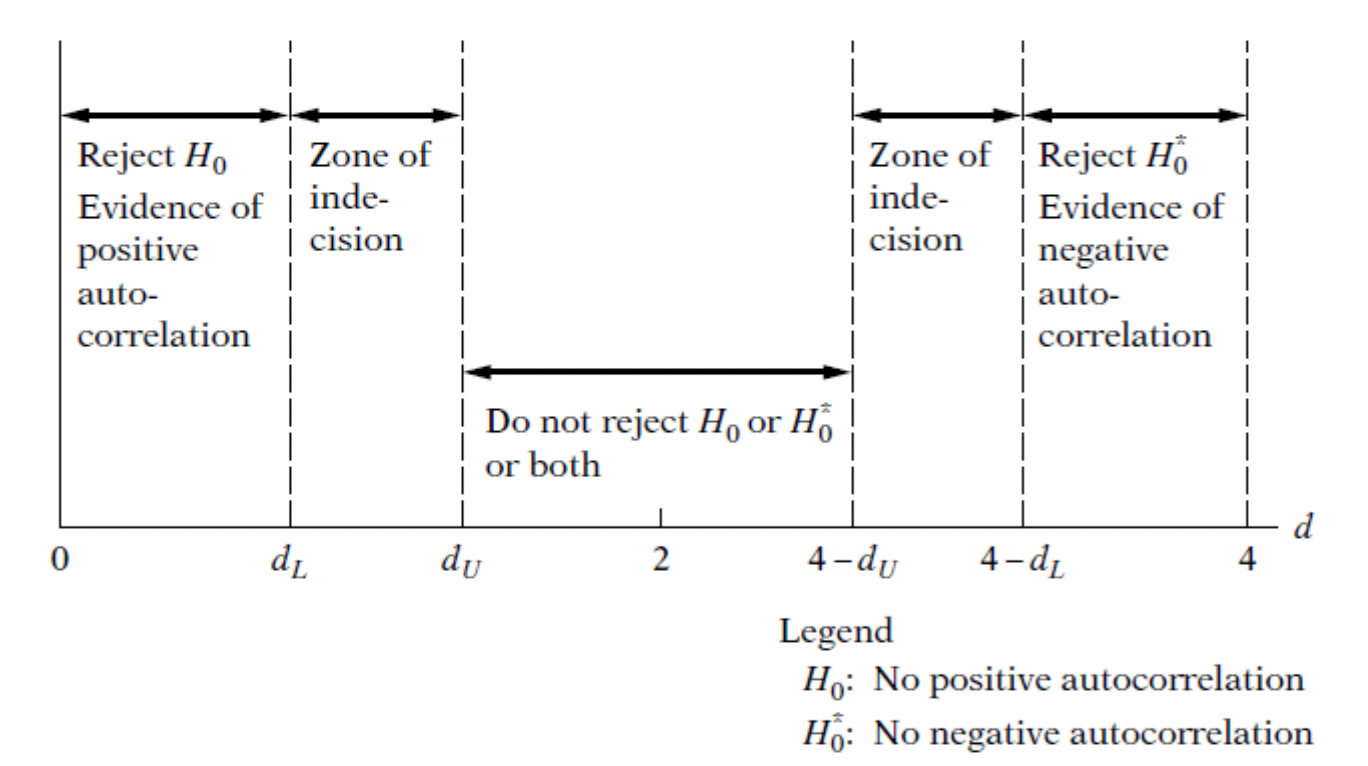
\includegraphics[width=10cm, height=8cm]{DW.png}
\end{block}
\end{frame}

\section{Estimateur Robuste de Newey West}

\frame{\tableofcontents[current]}


\begin{frame}{Estimateur Robuste de Newey West}
\begin{itemize}
\item Il existe une forme de correcteur robuste pour les problèmes d’autocorrélation des erreurs qui est une alternative au FGLS quand le nombre d’observations est assez élevé.
\item Cette correction est asymptotique.
\item C’est l’estimateur de la variance de Newey-West. 
\item L’intuition est la même que le correcteur de White, mais appliqué aux problèmes d’autocorrélation des erreurs.
\item En fait, le charme de l’estimateur de Newey-West c’est qu’il corrige pour \textbf{l’autocorrélation} ET \textbf{l’hétéroscédasticité des erreurs} (c’est ce qu’on appelle l’estimateur \textbf{HAC}).
\item Le correcteur de Newey West est déjà programmé dans les logiciels d’analyses de données comme Stata.
\end{itemize}
\end{frame}

\end{document}